\section{Studio dei processi}
Come già detto, un \textbf{processo software} è un insieme di attività atte alla creazione di un software, comprende almeno le quattro attività fondamentali e si sceglie in base al caso di studio. I vantaggi di una sua definizione sono evidenti: garantire uno standard lavorativo e di conseguenza un livello minimo di qualità del prodotto. Esistono numerosi processi software, dai più \textbf{prescrittivi}, caratterizzati da regole e fasi ben definite, ai più \textbf{adattivi}, che privilegiano flessibilità e adattamento ai cambiamenti.\par
Conoscere i modelli di processo è fondamentale per i \textbf{project manager}, poiché è compito loro decidere quale adottare considerando la tipologia del software da progettare. È un tema complesso, perché ha un enorme impatto sulla buona riuscita del progetto. Un secondo motivo per cui è bene conoscere i processi è uscire da quello di bruteforcing, conosciuto anche come \textbf{code and fix}, verosimilmente utilizzato da te fino all'avvento di questa materia. Si tratta di un modus operandi privo di analisi e progettazioni, il cui prodotto si crea esclusivamente per tentativi. È chiaro che non è un metodo adatto per progetti professionali, quindi nelle prossime sezioni analizzeremo le tipologie di processo più usate: a cascata, evolutivi, basati sulla configurazione e integrazione di componenti e agili.

%

\section{Modelli a cascata}
Storicamente, il modello \textbf{Waterfall} è il primo mai utilizzato in ambito di sviluppo software. Mette in cascata i passi tradizionali dello sviluppo di un sistema ed ogni fase produce un \textbf{deliverable}, il quale verrà usato come input di quella successiva, fino al termine del processo. Presenta i seguenti passi: \begin{itemize}
	\item \textbf{Studio della fattibilità}: Valutazione di fattibilità e convenienza in base al tempo e le risorse disponibili. Si stima inoltre il \textbf{return on investment} (ROI), ovvero il guadagno potenziale derivante dall'investimento nello sviluppo del software.
	\item \textbf{Definizione e analisi dei requisiti}: Raccolta delle richieste del cliente. Il deliverable è il \textbf{documento dei requisiti}, il quale fornisce i dettagli in merito alle funzionalità del programma. Può avere definizioni, specifiche o visualizzazioni grafiche.
	\item \textbf{Design del software}: La definizione delle componenti del sistema con le relative relazioni (\textbf{high-level design}) oppure la definizione interna di ogni componente (\textbf{low-level design}). Il deliverable è la specifica del design mediante un \textbf{linguaggio di modellazione unificato} (UML).
	\item \textbf{Implementazione del codice}: La scrittura effettiva del codice insieme al mandatorio unit testing. Ci sono diversi paradigmi di sviluppo, ma il deliverable rimane sempre il codice completo del programma.
	\item \textbf{Verifica del codice}: Il testing del codice con l'eventuale integrazione di soluzioni ai problemi. Il deliverable fornisce i dettagli sui test effettuati insieme ad un report.
	\item \textbf{Mantenimento del codice}: La costante manutenzione del software per la durata del suo ciclo di vita, come l'aggiunta di nuove feature, ottimizzazioni o di adattare il codice alle nuove tecnologie, come l'ultima versione di un sistema operativo.
\end{itemize}
\noindent I pregi dell'uso di questo metodo sono l'enfasi sull'analisi dei requisiti ed il progetto di sistema, perché prima di cominciare ci si assicura di aver determinato correttamente i bisogni del cliente e di averli definiti adeguatamente. Sebbene questo sia un processo solido, allo stesso tempo risulta rigido e monolitico, rendendo difficile contemplare cambiamenti al progetto in corso d'opera.\par
Per far fronte a questo problema di flessibilità sono stati ideati altri modelli ispirati al waterfall che implementano il concetto di feedback e interazioni durante lo sviluppo. Per esempio, nel \textbf{modello a cascata iterativo} si ha la possibilità di ritornare a una fase precedente in base al feedback dato dallo stakeholder, ottenuto di norma fornendo un prototipo. Un'altra variante è il \textbf{modello a V}, che dà molta enfasi al testing, mostrando anche come le loro attività siano collegate a quelle di analisi e progettazione. In questo paradigma, infatti, ogni controllo che non ha esito positivo porta a un rifacimento o modifica della fase associata, per poi riprendere il workflow da quella fase.\par
Sebbene questi due modelli abbiano apportato migliorie al waterfall, è evidente che siano ugualmente poco flessibili agli imprevisti. Nella maggior parte dei casi non è realistico che i requisiti rimangano gli stessi per quelli che potrebbero essere anni di lavoro. Per questo motivo sono stati ideati altri paradigmi di sviluppo software con alla base la possibilità di evolversi in base al feedback del cliente.
\begin{figure}[h]
	\centering
	\subcaptionbox{Modello a cascata}{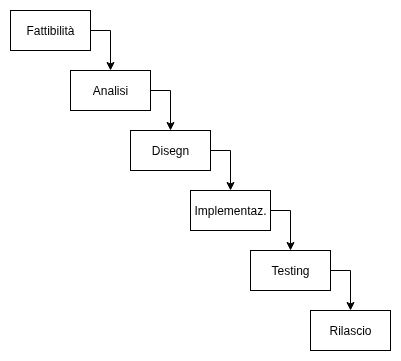
\includegraphics[width=0.45\linewidth]{Images/WaterfallModel.png}}
	\hfill
	\subcaptionbox{Modello a cascata iterativo}{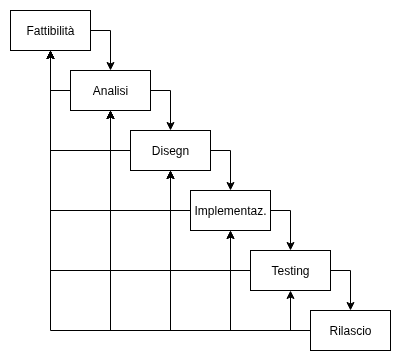
\includegraphics[width=0.45\linewidth]{Images/WaterfallIterationModel.png}}
	\hfill
	\subcaptionbox{Modello a V}{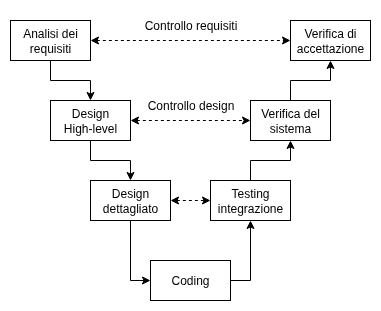
\includegraphics[width=0.45\linewidth]{Images/V-Model.png}}
\end{figure}

%

\section{Modelli evolutivi}
I \textbf{modelli evolutivi} si basano sull'idea di sviluppare una versione iniziale del software, incompleta ma funzionante, da sottoporre agli utenti e raffinare progressivamente tramite feedback, fino al raggiungimento delle funzionalità richieste.\par
Un primo esempio è dato dai \textbf{modelli di prototipizzazione}, la cui implementazione è data da prototipi del sistema, sui quali validare i requisiti. Se questo soddisfa le richieste degli utenti, può essere evoluto nel sistema finale; in alternativa, può essere scartato dopo aver chiarito i requisiti. Essendo spesso un artefatto temporaneo, il prototipo non viene sviluppato con particolare attenzione all'efficienza o alla qualità del codice; infatti sono usati strumenti e tecnologie per una rapida realizzazione.\par
Questo modello di sviluppo consente di raffinare al meglio i requisiti definiti dagli stakeholder e permette di rilevare errori di interpretazione molto facilmente. Tuttavia, si tratta di un processo dispendioso in termini di risorse fisiche e psichiche. In particolare, esiste il rischio di considerare il prototipo come prodotto finale, compromettendo la qualità del sistema e annullando i benefici della prototipizzazione. Per questa ragione i prototipi riguardano tendenzialmente funzionalità su cui il cliente ha fornito requisiti ambigui.
\begin{figure}[h]
	\centering
	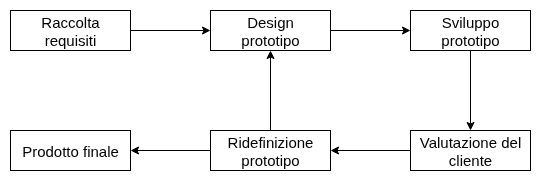
\includegraphics[width=0.8\linewidth]{Images/model_prototyping.png}
	\caption{Modello di prototipizzazione}
\end{figure}

\noindent Due altri modelli che consentono una rapida risposta alle richieste degli stakeholder e del mercato sono quelli \textbf{incrementali} e \textbf{iterativi}, che prevedono lo sviluppo di più release utilizzabili di cui solo l'ultima è completa. In particolare, per il primo si richiede di individuare le funzionalità fondamentali del software per il primo rilascio (qui si implementano tipicamente i requisiti a maggior valore per gli utenti), al quale saranno aggiunte altre funzioni con l'avvento delle successive release, fornendo versioni del software sempre più complete.\par
Per i modelli \textbf{iterativi}, invece, si sviluppa una versione iniziale del sistema che viene progressivamente migliorata e raffinata a ogni iterazione, sia in termini di funzionalità sia di qualità. Per esempio, si potrebbe sviluppare un word processor funzionante con una CLI, per poi fare una seconda release con una GUI.\par
I vantaggi di questi modelli risiedono nella possibilità di ottenere rapidamente versioni funzionanti del software, raccogliere feedback dagli stakeholder e adattare lo sviluppo di conseguenza, riducendo il rischio di errori nei requisiti e migliorando progressivamente il prodotto.\newline

\noindent Il principale modello di sviluppo evolutivo è il \textbf{modello a spirale}: si tratta di un approccio realistico per sistemi di grandi dimensioni, il quale si evolve insieme alle interazioni continue tra stakeholder e team operativo. È un workflow guidato dal rischio, inteso come una circostanza potenzialmente avversa in grado di compromettere lo sviluppo e la qualità del software.\par
Nel lavoro è necessario fare delle scelte, e, come per gli investimenti, comportano un rischio. Per questa ragione, bisogna valutare la gravità delle conseguenze e la probabilità che la circostanza si verifichi. Il modello presenta quattro fasi entro le quali si itera fino al raggiungimento del prodotto definitivo: \begin{itemize}
	\item \textbf{Pianificazione}: Determinazione degli obiettivi, alternative e vincoli da rispettare.
	\item \textbf{Analisi dei rischi}: Identificazione dei rischi, alternative ed eventuali risoluzioni.
	\item \textbf{Sviluppo del software}: Sviluppo del prodotto.
	\item \textbf{Convalida del cliente}: Revisione dei risultati da parte del committente.
\end{itemize}
\noindent I principali vantaggi risiedono nella grande flessibilità ai problemi, ma non è una soluzione universale e richiede una buona competenza nella valutazione dei rischi, perché in base alle conseguenze, potrebbe essere necessaria una significativa revisione del prodotto.
\begin{figure}[h]
	\centering
	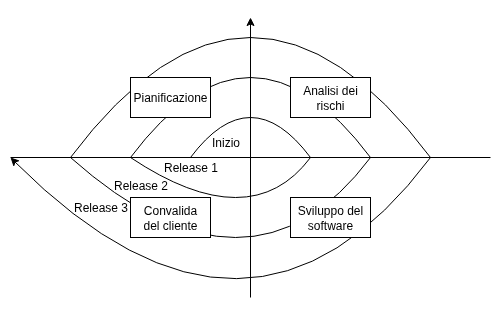
\includegraphics[width=0.8\linewidth]{Images/model_spiral.png}
	\caption{Modello a spirale}
\end{figure}

%

\section{Ulteriori approcci}
I modelli di sviluppo non si limitano solo ad essere guidati da un piano oppure dal feedback del cliente, bensì possono integrare idee di entrambi, come per l'\textbf{unified process}: un approccio per lo sviluppo di sistemi a oggetti con notazioni UML. È guidato dagli \textbf{use case} e incorpora alcune idee del modello a spirale, come i rilasci multipli dopo ogni fase e una forte enfasi sulla convalida del cliente, mantenendo però una struttura plan-driven. Il modello presenta quattro fasi: \begin{itemize}
	\item \textbf{Concezione}: Studio di fattibilità e definizione dei requisiti essenziali.
	\item \textbf{Elaborazione}: Studio del dominio applicativo e definizione dell'architettura del software.
	\item \textbf{Costruzione}: Design del prodotto, codifica e testing.
	\item \textbf{Transizione}: Utilizzo del software nel contesto applicativo da parte di utenti fidati.
\end{itemize}
\noindent Ognuna di queste fasi presenta cinque workflow: \textbf{Requisiti}, \textbf{Analisi}, \textbf{Design}, \textbf{Codifica} e \textbf{Testing}.
\begin{figure}[h]
	\centering
	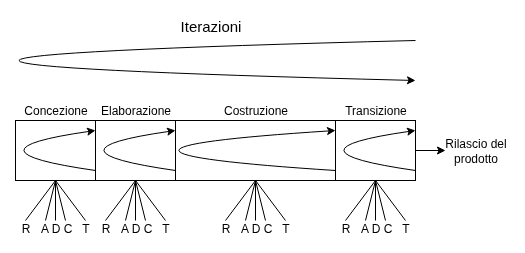
\includegraphics[width=1\linewidth]{Images/model_UP.png}
\end{figure}

\noindent Un altro approccio con una diversa filosofia è dato dallo \textbf{sviluppo basato sui componenti}, la cui idea fondamentale è la minimizzazione di riscrittura di nuovo codice, riutilizzando componenti già a disposizione, piuttosto che scriverne di nuovi. Idee come questa sono supportate dalla presenza di un mercato degli asset, dal quale si attinge. Presenta le seguenti fasi: \begin{itemize}
	\item \textbf{Specifica dei requisiti}
	\item \textbf{Analisi dei componenti}
	\item \textbf{Modifica delle richieste}
	\item \textbf{Design orientato al riutilizzo}
	\item \textbf{Sviluppo e integrazione}
	\item \textbf{Convalida del sistema}
\end{itemize}
\noindent Lo sviluppo inizia dunque dalla ricerca dei componenti in base alle richieste del cliente; questi sono forniti dal marketplace, aziende terze o da progetti open-source. Eventualmente, se non rispettano i requisiti, è possibile ridefinirli con il committente oppure cercare di sostituirli; dopodiché si procede con l'implementazione ed infine la validazione.\par
Il vantaggio principale è il risparmio di tempo: affidandoci a prodotti già scritti e funzionanti si riducono costi totali e rischi. Tuttavia, non è sempre facile allineare i desideri del committente con le componenti a disposizione, spesso non modificabili. Inoltre, essendo dipendenti da terzi, le parti utilizzate potrebbero venire aggiornate al di fuori dal controllo del team.\par
Esistono infine modelli basati su metodi formali, dove si richiede che venga tutto definito in modo rigoroso e con prove matematiche, come il \textbf{modello trasformazionale}. La specifica viene formalizzata e guida lo sviluppo fino ad arrivare all'implementazione. Risulta vantaggioso perché ci consente di provare con (quasi) assoluta certezza il funzionamento del codice grazie alle relative dimostrazioni.\newline

\noindent Presentiamo qualche cenno sul workflow più utilizzato in ambito lavorativo odierno: i \textbf{metodi agili}. Qui si pone meno enfasi sulla documentazione formale, privilegiando la comunicazione diretta e la produzione di software funzionante per garantire una maggiore flessibilità ai cambi repentini del mercato e degli stakeholder. La filosofia di questi modelli pone la soddisfazione del cliente come obiettivo più importante, rispetto a seguire un piano. Presentano le seguenti caratteristiche: \begin{itemize}
	\item \textbf{Ciclo rapido e consegne frequenti}: Ogni iterazione produce un incremento funzionante del software, rilasciato in tempi brevi.
	\item \textbf{Progettazione semplice}: Sviluppo orientato alla realizzazione delle funzionalità essenziali, evitando complessità non necessarie.
	\item \textbf{Refactoring}: Il codice è costantemente ristrutturato per renderlo quanto più chiaro possibile. Il codice dovrebbe quindi "commentarsi da solo".
	\item \textbf{Meeting di riflessione}: Incontri periodici per pianificare il lavoro, monitorare l'avanzamento e riflettere sui miglioramenti del processo.
	\item \textbf{Conoscenza tacita e implicita}: Si privilegia lo scambio di informazioni tra i membri del team rispetto a documentazione formale eccessiva. (Pratica dubbia, ma efficiente sul breve termine).
	\item \textbf{Co-Location}: Stretta interazione con gli stakeholder, idealmente con una presenza costante o facilmente accessibile.
\end{itemize}
\noindent È evidente che questi metodi presentano alcune criticità, tra cui una maggiore dipendenza dalla collaborazione tra i membri del team, difficoltà nella manutenzione in caso di documentazione insufficiente e da un punto di vista legale, data la flessibilità (e quindi ambiguità) del contratto.